% !TeX spellcheck = cs_CZ
\begin{mathexam}{Ortogonální projekce v prostoru \(\mathcal{R}^3\)}{exam012}
    Je-li \(\mathbf{P}\) matice ortogonální projekce v prostoru \(\mathcal{R}^3\) na nějaký 
    podprostor \(\mathcal{U}\) (\(\mathcal{U}\) je tedy buď rovina nebo přímka procházející 
    počátkem), pak pro každý vektor \(\mathbf{u}\in\mathcal{U}\) platí \(\mathbf{Pu} = 
    \mathbf{u}\), všechny vektory z \(\mathcal{U}\) (s výjimkou nulového vektoru \(\Theta\)) 
    jsou vlastními vektory matice $\mathbf{P}$ příslušné vlastnímu číslu \(\lambda\). Prostor 
    \(\mathrm{U}^\bot\) je roven jádru projekce (nulovému prostoru matice \(\mathbf{P}\)), 
    a tedy každý vektor z ortogonálního doplňku \(\mathcal{U}\) (s výjimkou \(\Theta\)) je 
    vlastním vektorem příslušným k vlastnímu číslu \(0\).

    {\centering
      \captionsetup{type=figure}
      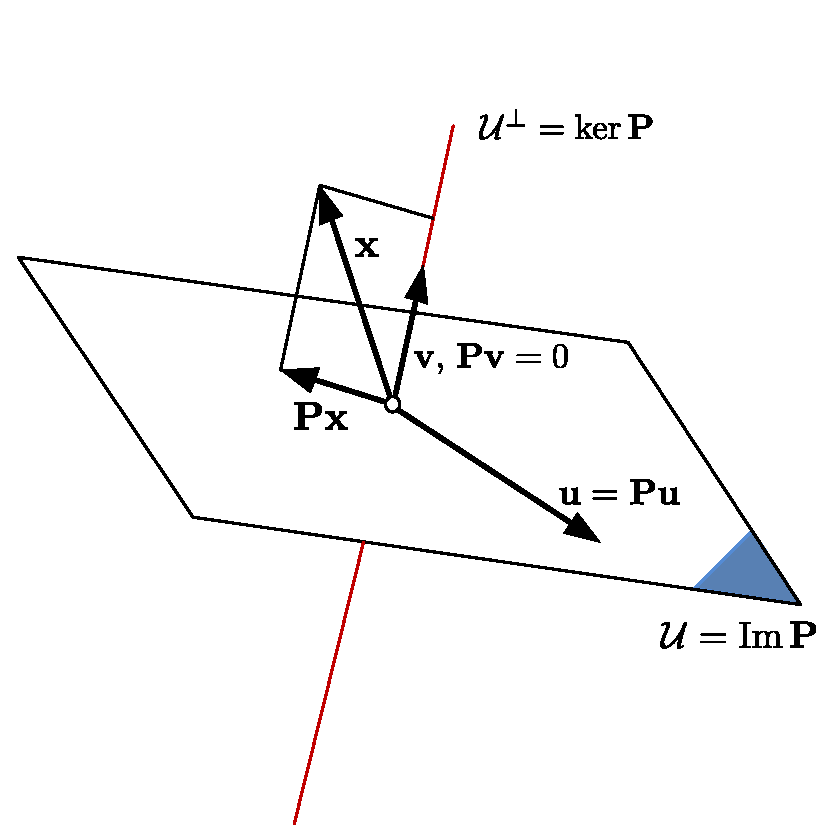
\includegraphics[width=0.5\linewidth]{mai_fig024.pdf}
      \captionof{figure}{K příkladu \ref{mai:exam012}}
      \label{MAI:FIG016}
      \par}

\end{mathexam}